\documentclass[11pt,twoside,reqno]{amsart}
\usepackage{amssymb, amsmath, enumerate, palatino, hyperref}
\usepackage[normalem]{ulem}
%\usepackage{fullpage}
\usepackage[margin=1in]{geometry}
\usepackage[T1]{fontenc}
\renewcommand{\labelitemi}{\guillemotright}
\usepackage{mathrsfs}
%--------------------------------
% Kees' imports
%--------------------------------
\usepackage{physics}
\usepackage{tensor}
\usepackage{mathtools}
\usepackage{xcolor}
\usepackage{siunitx}
\usepackage{empheq}
\usepackage{tensor}


\theoremstyle{plain}
\newtheorem{prop}{Proposition}%[section]
\newtheorem{lemma}[prop]{Lemma}
\newtheorem{thm}[prop]{Theorem}
\newtheorem{obs}[prop]{Observation}
\newtheorem{app}[prop]{Application}
\newtheorem*{MainThm}{Main Theorem}
\newtheorem{cor}[prop]{Corollary}
\newtheorem{conj}[prop]{Conjecture}
\theoremstyle{remark}
\newtheorem{rmk}[prop]{Remark}
\theoremstyle{definition}
\newtheorem{prob}{Problem}
\newtheorem{bonus}[prop]{Bonus Problem}
\theoremstyle{remark}
\newtheorem{exc}{Exercise}
\newtheorem*{soln}{Solution}
\theoremstyle{definition}
\newtheorem{ex}[prop]{Example}
\theoremstyle{definition}
\newtheorem{defn}[prop]{Definition}

\newcommand{\RR}{\mathbb{R}}
\newcommand{\ZZ}{\mathbb{Z}}
\newcommand{\CC}{\mathbb{C}}
\newcommand{\NN}{\mathbb{N}}
\newcommand{\QQ}{\mathbb{Q}}

\newcommand{\Aut}{\operatorname{Aut}}

\newcommand{\defeq}{:=}

\renewcommand{\Re}{\operatorname{Re}}

%--------------------------------
% Kees' commands
%--------------------------------
\makeatletter
\newcommand{\subalign}[1]{%
  \vcenter{%
    \Let@ \restore@math@cr \default@tag
    \baselineskip\fontdimen10 \scriptfont\tw@
    \advance\baselineskip\fontdimen12 \scriptfont\tw@
    \lineskip\thr@@\fontdimen8 \scriptfont\thr@@
    \lineskiplimit\lineskip
    \ialign{\hfil$\m@th\scriptstyle##$&$\m@th\scriptstyle{}##$\hfil\crcr
      #1\crcr
    }%
  }%
}
\makeatother

\newcommand{\allspace}{{\substack{\text{all}\\\text{space}}}}

\newcommand{\DD}{\mathbb{D}}
\renewcommand{\AA}{\mathbb{A}}
\newcommand{\VV}{\mathbb{V}}
\newcommand{\LL}{\mathbb{L}}
\newcommand{\BB}{\mathbb{B}}
\renewcommand{\SS}{\mathbb{S}}
\newcommand{\HH}{\mathbb{H}}

\renewcommand{\l}{\ell}

\newcommand{\PB}{\mathrm{PB}}

\newcommand{\cL}{\mathcal{L}}
\newcommand{\cE}{\mathcal{E}}
\newcommand{\cH}{\mathcal{H}}
\newcommand{\cC}{\mathcal{C}}
\newcommand{\cA}{\mathcal{A}}
\newcommand{\cI}{\mathcal{I}}
\newcommand{\cM}{\mathcal{M}}
\newcommand{\cO}{\mathcal{O}}

\newcommand{\sgn}{\mathrm{sgn}}

\newcommand{\LIPS}{\mathrm{LIPS}}
\newcommand{\zcut}{z_\mathrm{cut}}
\newcommand{\mMDT}{\mathrm{mMDT}}

\newcommand{\Ei}{\mathrm{Ei}}
\newcommand{\Li}{\mathrm{Li}}

\newcommand{\arctanh}{\mathrm{arctanh}}
\newcommand{\arcsinh}{\mathrm{arcsinh}}

\def\beq#1\eeq{\begin{equation}#1\end{equation}}
\def\bal#1\eal{\begin{align}#1\end{align}}

\title{Calculating the soft function}
\author{Kees Benkendorfer}
\date{24 February 2021}

\begin{document}
\maketitle

\tableofcontents

\section{Setup}
	We wish to calculate the resolved soft function $S_R(\rho - \zcut)$ which describes soft radiation which passes the groomer due to proximity to the resolved gluon. If the resolved emission occurs at an angle $\theta$ from the quark axis, then any radiation at smaller angles will pass the groomer. A schematic of this situation is displayed in Fig.~\ref{fig:schematic}.

	The goal is to calculate the first-order term in an expansion of $S_R$. We can then use renormalization group evolution in conjunction with the other first-order results of functions in the factorization equation to achieve an all-orders calculation of the cross section.

	Let the resolved gluon have momentum $k_g$, the quark lie along direction $n_q = (1, 0, 0, 1)$, and consider an extra-soft gluon with momentum $k$. If the extra-soft gluon is closer to the quark, then its dominant contribution to the jet mass $\rho$ will come from its interaction with the quark:
	\begin{equation}
		\rho = \frac{4 k^+}{Q}
	\end{equation}
	where $k^{\pm} = k^0 \mp k_z$ are light-cone coordinates defined with respect to the quark axis. If the extra-soft gluon is closer to the resolved gluon, then its contribution to the jet mass from the quark interaction has already been accounted for in the contribution of the resolved gluon. The leading-order contribution from the new gluon therefore comes with its interaction with the resolved gluon. If $n_g$ is the direction of the resolved gluon, then the contribution is
	\begin{equation}
		\rho = \frac{4 k \cdot n_g}{Q} = \frac{4 k \cdot k_g}{E_g Q}
	\end{equation}
	with $E_g$ the energy of the resolved gluon.

	Notice that the angle between the extra-soft gluon and the quark is given by
	\begin{equation}
		1 - \cos\theta_{gq} = \frac{k^+}{k^0}
	\end{equation}
	while the angle between the extra-soft gluon and the resolved gluon is
	\begin{equation}
		1 - \cos\theta_{gg} = \frac{k \cdot n_g}{k^0}.
	\end{equation}
	The case in which the extra-soft gluon is closer to the quark is the case in which $\theta_{gq} < \theta_{gg}$, so $1 - \cos\theta_{gq} < 1 - \cos\theta_{gg}$ and, in turn $k^+ < k \cdot n_g$. Therefore, the total measurement function is
	\begin{equation}
		\delta_\rho = \Theta(k^+ - k\cdot n_g)\,\delta\qty(\rho - \frac{4k^+}{Q}) + \Theta(k\cdot n_g - k^+)\,\delta\qty(\rho - \frac{4k\cdot n_g}{Q}).
	\end{equation}

	\begin{figure}\label{fig:schematic}
		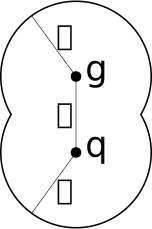
\includegraphics[width=0.15\textwidth]{figures/head_on_schematic.pdf}
		\caption{Schematic head-on view of emissions according to the jet groomer. Radiation within the peanut-shaped region will pass the grooming algorithm.}
	\end{figure}

	We also need to impose the kinematic constraint that the gluon is in the peanut-shaped region of Fig.~\ref{fig:schematic}. Saying that the gluon is in the region is equivalent to saying that it is not outside the region. The gluon is outside of the quark's radius of influence if
	\begin{equation}
		\frac{k^+}{k^0} = 1 - \cos\theta_{gq} > 1 - \cos\theta = n_g \cdot n_q.
	\end{equation}
	On the other hand, the gluon is outside the resolved gluon's radius of influence if
	\begin{equation}
		\frac{k \cdot n_g}{k^0} = 1 - \cos\theta_{gg} > 1 - \cos\theta = n_g \cdot n_q.
	\end{equation}
	Therefore, the grooming restriction is
	\begin{equation}
		\Theta_{\mMDT} = 1 - \Theta(k^+ - k^0 n_g \cdot n_q)\,\Theta(k \cdot n_g - k^0 n_g \cdot n_q).
	\end{equation}

	The matrix element accounts for the possibility that the gluon be emitted from any pairs of resolved particles {\color{red}\textbf{[TODO: need to sort out prefactors, include color matrices. Also it's not actually a sum]}}
	\begin{equation}
		\abs{\cM}^2 = \sum_{i < j} \frac{n_i \cdot n_j}{(n_i \cdot k)(n_j \cdot k)}
	\end{equation}
	where $i, j$ range over all pairs of resolved particles. Each term of the matrix element corresponds to a separate soft function. For now, we will focus on the first term
	\begin{equation}
		\abs{\cM_{q\bar q}}^2 = \frac{n_q \cdot n_{\bar q}}{(n_q \cdot k)(n_{\bar q}\cdot k)} = \frac{2}{k^+ k^-}
	\end{equation}
	with $n_{\bar q} = (1, 0, 0, -1)$ the antiquark direction. {\color{red}\textbf{[TODO: need to handle other soft functions]}}

	Finally, phase space in $d$ dimensions takes the usual form
	\begin{equation}
		d\Pi = \frac{d^d k}{(2\pi)^d} 2\pi\,\delta\qty(k^2)\,\Theta(k^+)\,\Theta(k^- - k^+).
	\end{equation}
	Notice that we are enforcing the gluon to be emitted in the hemisphere with the quark by requiring $k^- - k^+$. We will multiply the result at the end by a factor of $2$ to account for the case where the gluons are emitted in the other hemisphere. Note that we are only scanning over the momentum of the extra-soft gluon: under the assumption that this gluon is softer than the resolved gluon, this emission does not influence the momentum of the quarks or resolved gluon.

	Putting everything together, we find
	\begin{equation}\label{eq:soft integral}
	\begin{aligned}
		S_R(\rho - \zcut) = 2 \int& \frac{d^d k}{(2\pi)^{d-1}} \, \delta\qty(k^2)\,\Theta(k^+)\,\Theta(k^- - k^+) \,\frac{2}{k^+ k^-} \\
		&\times \qty[\Theta(k^+ - k\cdot n_g)\,\delta\qty(\rho - \frac{4k^+}{Q}) + \Theta(k\cdot n_g - k^+)\,\delta\qty(\rho - \frac{4k\cdot n_g}{Q})] \\
		&\times \qty[1 - \Theta(k^+ - k^0 n_g \cdot n_q)\,\Theta(k \cdot n_g - k^0 n_g \cdot n_q)].
	\end{aligned}
	\end{equation}

\section{Coordinate choice}
	Now we need to determine which coordinates in which to work. Notice that, physically, there is an axial symmetry to the problem: nothing depends on the angle of the resolved emission about the quark axis. Therefore, we might define our momenta in terms of their transverse momentum, pseudorapidity, and angle about the axis. To get from Cartesian $(p_x, p_y, p_z)$ to this detector coordinate system $(p_\perp, \phi, \eta)$, we use the following transformations:
	\begin{equation}
	\begin{aligned}
		p_x &= p_\perp \cos\phi & p_y &= p_\perp \sin\phi & p_z &= p_\perp \sinh\eta & p_0 &= p_\perp \cosh\eta \\
		p_\perp &= \sqrt{p_x^2 + p_y^2} & \phi &= \arctan(\frac{p_y}{p_x}) & \eta &= \arctanh\qty(\frac{p_z}{\abs{\vb{p}}}).
	\end{aligned}
	\end{equation}

	Under this transformation, the extra-soft gluon has momentum
	\begin{equation}
		k = (k_0, k_\perp, \phi_k, \eta_k).
	\end{equation}
	The resolved gluon is fixed in space from the perspective of the extra-soft gluon, so we can write it in whichever coordinates are convenient. Let us pick spherical coordinates, where the gluon momentum has an azimuthal angle $\phi_g$ and an angle $\theta_g$ from the jet axis
	\begin{equation}
		k_g = (k_0, r, \theta, \phi) = (E_g, E_g, \theta_g, \phi_g)
	\end{equation}
	and hence direction vector
	\begin{equation}
		n_g = \qty(1, 1, \theta_g, \phi_g).
	\end{equation}
	Finally, without loss of generality, we can define our coordinate axis so that the resolved emission is at angle $\phi_g = 0$, thereby setting
	\begin{equation}
	\begin{aligned}
		k_g &= (E_g, E_g, \theta_g, 0) & n_g &= (1, 1, \theta_g, 0).
	\end{aligned}
	\end{equation}

	Now we can transform each term of Eq.~\ref{eq:soft integral}. First, notice that
	\begin{equation}
		k^+ = k_0 - k_z = k_\perp \qty(\cosh\eta_k - \sinh\eta_k) = k_\perp e^{-\eta_k},
	\end{equation}
	and similarly
	\begin{equation}
		k^- = k_\perp e^{\eta_k}.
	\end{equation}
	Hence, the restriction $k^+ > 0$ becomes $k_\perp > 0$ and $k^- > k^+$ becomes $\eta_k > 0$. That is,
	\begin{equation}
		\Theta(k^+)\,\Theta(k^- - k^+) = \Theta(k_\perp)\,\Theta(\eta_k).
	\end{equation}
	The first term in the matrix element is then simply
	\begin{equation}
		\abs{\cM}^2 = \frac{2}{k^+ k^-} = \frac{2}{k_\perp^2}.
	\end{equation}

	Next comes the measurement function. First notice that (in Cartesian coordinates)
	\begin{equation}
	\begin{aligned}
		k \cdot n_g &= (k_\perp \cosh\eta_k, k_\perp \cos\phi_k, k_\perp \sin\phi_k, k_\perp\sinh\eta_k) \cdot (1, \sin\theta_g, 0, \cos\theta_g) \\
		&= k_\perp \qty[\cosh\eta_k - \cos\phi_k \sin\theta_g - \sinh\eta_k \cos\theta_g].
	\end{aligned}
	\end{equation}
	Therefore
	\begin{equation}
	\begin{aligned}
		\Theta(k^+ - k\cdot n_g) &= \Theta\qty(\cos\phi_k \sin\theta_g - (1- \cos\theta_g)\sinh\eta_k) \\
		&= \Theta\qty(\cos\phi_k\frac{\sin\theta_g}{1 - \cos\theta_g} - \sinh\eta_k) \\
		&= \Theta\qty(\cos\phi_k\cot\frac{\theta_g}{2} - \sinh\eta_k)
	\end{aligned}
	\end{equation}
	and
	\begin{equation}
		\Theta(k\cdot n_g - k^+) = \Theta\qty(\sinh\eta_k - \cos\phi_k\cot\frac{\theta_g}{2}).
	\end{equation}
	The full measurement function is then
	\begin{equation}
	\begin{aligned}
		\delta_\rho &= \Theta\qty(\cos\phi_k\cot\frac{\theta_g}{2} - \sinh\eta_k)\,\delta\qty(\rho - \frac{4 k_\perp e^{-\eta_k}}{Q}) \\
			&\quad+ \Theta\qty(\sinh\eta_k - \cos\phi_k\cot\frac{\theta_g}{2})\, \delta\qty(\rho - \frac{4 k_\perp}{Q}\qty[\cosh\eta_k - \cos\phi_k\sin\theta_g - \sinh\eta_k\cos\theta_g]).
	\end{aligned}
	\end{equation}

	Finally, we have the mMDT groomer. Notice that
	\begin{equation}
		\Theta\qty(k^+ - k^0 n_g \cdot n_q) = \Theta(\cos\theta_g - \tanh\eta_k)
	\end{equation}
	and
	\begin{equation}
		\Theta\qty(k\cdot n_g - k^0 n_g \cdot n_q) = \Theta\qty(\cot\theta_g - e^{\eta_k}\cos\phi_k).
	\end{equation}
	Therefore,
	\begin{equation}
		1 - \Theta(k^+ - k^0 n_g \cdot n_q)\,\Theta(k \cdot n_g - k^0 n_g \cdot n_q) = 1 - \Theta(\cos\theta_g - \tanh\eta_k)\,\Theta\qty(\cot\theta_g - e^{\eta_k}\cos\phi_k).
	\end{equation}

	Putting everything together so far, we have
	\begin{equation}
	\begin{aligned}
		S_R = 2 \int &\frac{d^d k}{(2\pi)^{d-1}} \delta(k^2)\,\Theta(k_\perp) \,\Theta(\eta_k)\,\frac{2}{k_\perp^2} \\
			&\times \Bigg[ \Theta\qty(\cos\phi_k\cot\frac{\theta_g}{2} - \sinh\eta_k)\,\delta\qty(\rho - \frac{4 k_\perp e^{-\eta_k}}{Q}) \\
			&\qquad+ \Theta\qty(\sinh\eta_k - \cos\phi_k\cot\frac{\theta_g}{2})\, \delta\qty(\rho - \frac{4 k_\perp}{Q}\qty[\cosh\eta_k - \cos\phi_k\sin\theta_g - \sinh\eta_k\cos\theta_g])\Bigg] \\
			&\times \qty[1 - \Theta(\cos\theta_g - \tanh\eta_k)\,\Theta\qty(\cot\theta_g - e^{\eta_k}\cos\phi_k)].
	\end{aligned}
	\end{equation}

	The last thing to evaluate is the phase space measure. We wish to convert
	\begin{equation}
		dk_0 dk_z \,d^{d-2} k_\perp\,\delta(k^2) \to dk_0 d\eta_k\,d^{d-2}dk_\perp\,\delta(k^2)
	\end{equation}
	where $k_\perp$ represents the off-axis components of $k$ in $d-2$ dimensions. With $d = 4 - 2\epsilon$, we can write this in spherical coordinates as
	\begin{equation}
		d^{d-2}k_\perp = k_\perp^{d-3} d k_\perp\,\sin^{-2\epsilon}\phi_k\,d\phi_k \,d\Omega_{d-2}
	\end{equation}
	with $\Omega_{d-2}$ the solid angle of the $d-2$ dimensional sphere {\color{red}\textbf{[TODO: currently using wrong dimension for solid angle]}}. Integrating over this solid angle yields \cite{schwartz_quantum_2014}
	\begin{equation}
		\int d\Omega_{d-2} = \frac{2\pi^{(d-2)/2}}{\Gamma(\frac{d-2}{d})} = \frac{2\pi^{1-\epsilon}}{\Gamma(1 - \epsilon)}.
	\end{equation}
	Thus, we find that
	\begin{equation}
		d^{d-2}k_\perp = dk_\perp d\phi_k \,k_\perp^{d-3}\sin^{-2\epsilon}\phi_k\,\frac{2\pi^{1-\epsilon}}{\Gamma(1-\epsilon)}.
	\end{equation}
	Now also notice that
	\begin{equation}
		\delta(k^2) = \delta\qty(k_0^2 - k_\perp^2 - k_z^2) = \delta\qty(k_0^2 - k_\perp^2 \cosh^2\eta_k).
	\end{equation}
	This simplifies to
	\begin{equation}
		\delta\qty(k_0^2 - k_\perp^2 \cosh^2\eta_k) = \frac{1}{2k_\perp \cosh\eta_k}\delta\qty(k_0 - k_\perp \cosh\eta_k).
	\end{equation}
	Therefore, we can integrate out $k_0$ (notice that we have sneakily already applied the delta function where $k_0$ appeared earlier):
	\begin{equation}
		\int dk_0 \delta(k^2) = \frac{1}{2k_\perp \cosh\eta_k}.
	\end{equation}
	Finally, we need to account for the Jacobian in the $(k_0, k_z)$ transformation:
	\begin{equation}
		\frac{\partial(k_0, k_z)}{\partial(k_0, \eta_k)} = \mqty(
		1 & 0 \\ 
		0 & k_\perp \cosh\eta_k).
	\end{equation}
	The standard Jacobian factor is then the determinant (in absolute value)
	\begin{equation}
		dk_0 dk_z = k_\perp \cosh\eta_k \,dk_0 d\eta_k.
	\end{equation}
	All together, the phase space measure is
	\begin{equation}
	\begin{aligned}
		\int \frac{d^d k}{(2\pi)^{d-1}}\,\delta(k^2) &= \frac{\pi^{1-\epsilon}}{(2\pi)^{3-2\epsilon}\Gamma(1 - \epsilon)}\int dk_\perp d\phi_k d\eta_k \, k_\perp^{-1-2\epsilon} \sin^{-2\epsilon}\phi_k \\
		&= \frac{(4\pi)^\epsilon}{8\pi^2 \Gamma(1-\epsilon)} \int dk_\perp d\phi_k d\eta_k\,k_\perp^{-1-2\epsilon} \sin^{-2\epsilon}\phi_k.
	\end{aligned}
	\end{equation}
	Under the modified minimal subtraction scheme, we will set $(4\pi)^\epsilon \to 1$ (and will also set $\gamma_E \to 0$ as it comes up). The full integral is now
	\begin{equation}
	\boxed{
	\begin{aligned}
		S_R = \frac{1}{2\pi^2\Gamma(1 - \epsilon)} \int& dk_\perp d\phi_k d\eta_k\, k_\perp^{-1-2\epsilon} \sin^{-2\epsilon}\phi_k \, \Theta(k_\perp)\Theta(\eta_k) \\
		&\times \Bigg[ \Theta\qty(\cos\phi_k\cot\frac{\theta_g}{2} - \sinh\eta_k)\,\delta\qty(\rho - \frac{4 k_\perp e^{-\eta_k}}{Q}) \\
			&\qquad+ \Theta\qty(\sinh\eta_k - \cos\phi_k\cot\frac{\theta_g}{2})\, \delta\qty(\rho - \frac{4 k_\perp}{Q}\qty[\cosh\eta_k - \cos\phi_k\sin\theta_g - \sinh\eta_k\cos\theta_g])\Bigg] \\
			&\times \qty[1 - \Theta(\cos\theta_g - \tanh\eta_k)\,\Theta\qty(\cot\theta_g - e^{\eta_k}\cos\phi_k)].
	\end{aligned}
	}
	\end{equation}

\section{Evaluating the integral}
\subsection{Near the resolved gluon}
	Let us first evaluate the integral when
	\begin{equation}
		\cos\phi_k \cot\frac{\theta_g}{2} > \sinh\eta_k.
	\end{equation}
	In this scenario, the measurement delta function transforms as
	\begin{equation}
		\delta\qty(\rho - \frac{4k_\perp e^{-\eta_k}}{Q}) = \frac{Q e^{\eta_k}}{4}\delta\qty(k_\perp - \frac{\rho\,Q e^{\eta_k}}{4}).
	\end{equation}
	Then we can integrate out $k_\perp$ to find
	\begin{equation}
	\begin{aligned}
		S_R^I = \frac{1}{2\pi^2\Gamma(1-\epsilon)} \frac{1}{\rho^{1+2\epsilon}} \qty(\frac{Q}{4})^{-2\epsilon} \int& d\phi_k d\eta_k \,e^{-2\epsilon\eta_k} \sin^{-2\epsilon}\phi_k\,\Theta(\eta_k) \Theta\qty(\cos\phi_k\cot\frac{\theta_g}{2} - \sinh\eta_k) \\
		&\times \qty[1 - \Theta(\cos\theta_g - \tanh\eta_k)\Theta(\cot\theta_g - e^{\eta_k}\cos\phi_k)].
	\end{aligned}
	\end{equation}
	From here, notice that $\eta_k$ is bounded above, so the integral does not diverge; we can therefore set $\epsilon = 0$, which yields
	\begin{equation}\label{eq:gluon integral setup}
	\begin{aligned}
		S^I_R = \frac{1}{2\pi^2}\frac{1}{\rho} \int d\phi_k d\eta_k&\,\Theta(\eta_k)\Theta\qty(\cos\phi_k \cot\frac{\theta_g}{2} - \sinh\eta_k) \\
		&\times \qty[1 - \Theta(\cos\theta_g - \tanh\eta_k)\Theta(\cot\theta_g - e^{\eta_k}\cos\phi_k)].
	\end{aligned}
	\end{equation}
	The first $\eta_k$ integral is straightforward:
	\begin{equation}
		\int d\eta_k \Theta(\eta_k)\Theta\qty(\cos\phi_k \cot\frac{\theta_g}{2} - \sinh\eta_k) = \Theta\qty(\arcsinh\qty(\cos\phi_k \cot\frac{\theta_g}{2}))\arcsinh\qty(\cos\phi_k \cot\frac{\theta_g}{2}).
	\end{equation}
	Notice that since $\cot(\theta_g/2) > 0$ for $0 < \theta_g < \pi/2$,
	\begin{equation}
		\arcsinh\qty(\cos\phi_k \cot\frac{\theta_g}{2}) > 0 \iff \cos\phi_k > 0 \iff 0 < \phi_k < \frac{\pi}{2}
	\end{equation}
	if $\phi_k$ is restricted to $[0, 2\pi)$ {\color{red}\textbf{[Why can $\phi_k$ not range from $0$ to $2\pi$? Andrew said $0$ to $\pi$ but this is unclear to me]}}. The $\phi_k$ integral to solve is then
	\begin{equation}
		\int d\phi_k \,\Theta(\phi_k)\Theta\qty(\frac{\pi}{2} - \phi_k)\arcsinh\qty(\cos\phi_k\cot\frac{\theta_g}{2}).
	\end{equation}
	Try as I might, this integral seems fairly intractable {\color{red}\textbf{[Is this so?]}}, so we'll leave it as is. Thus, we have
	\begin{equation}\label{eq:gluon first integral}
	\begin{aligned}
		S_R^I = \frac{1}{2\pi^2\rho} \Bigg[ &\int_0^{\pi/2} d\phi_k \,\arcsinh\qty(\cos\phi_k\cot\frac{\theta_g}{2}) \\
			& - \int d\phi_k d\eta_k \Theta(\eta_k)\Theta\qty(\cos\phi_k \cot\frac{\theta_g}{2} - \sinh\eta_k)\Theta(\cos\theta_g - \tanh\eta_k)\Theta(\cot\theta_g - e^{\eta_k}\cos\phi_k)\Bigg]
	\end{aligned}
	\end{equation}

	The bounds on the second integral simplify as follows:
	\begin{equation}
	\begin{aligned}
		\Theta\Big(\cos\phi_k &\cot\frac{\theta_g}{2} - \sinh\eta_k\Big)\Theta(\cos\theta_g - \tanh\eta_k)\Theta(\cot\theta_g - e^{\eta_k}\cos\phi_k) \\
		&= \Theta\qty(1 - 2\cos\phi_k - \tan^2\frac{\theta_g}{2}) \Theta\qty(\arcsinh\qty(\cos\phi_k \cot\frac{\theta_g}{2}) - \eta_k) \\
			&\qquad+ \Theta\qty(2\cos\phi + \tan^2\frac{\theta_2}{2} - 1)\Theta\qty(\log(\cot\theta_g \sec\phi_k) - \eta_k).
	\end{aligned}
	\end{equation}
	Performing the $\eta_k$ integral is straightforward:
	\begin{equation}
	\begin{aligned}
		I = \int d\phi_k \, \Bigg[&\Theta\qty(1 - 2\cos\phi_k - \tan^2\frac{\theta_g}{2})\Theta\qty(\arcsinh\qty(\cos\phi_k \cot\frac{\theta_g}{2})) \arcsinh\qty(\cos\phi_k \cot\frac{\theta_g}{2}) \\
			&\qquad+ \Theta\qty(2\cos\phi + \tan^2\frac{\theta_2}{2} - 1)\Theta\qty(\log(\cot\theta_g \sec\phi_k))\log(\cot\theta_g \sec\phi_k) \Bigg].
	\end{aligned}
	\end{equation}
	Now, to handle the first term, notice that
	\begin{equation}
		\arcsinh\qty(\cos\phi_k \cot\frac{\theta_g}{2}) > 0 \implies \cos\phi_k \cot\frac{\theta_g}{2} > 0.
	\end{equation}
	Since $\cot(\theta_g/2) > 0$ for all $0 < \theta_g < \pi/2$, we therefore require $\cos\phi_k > 0$, or $0 < \phi_k < \pi/2$. Hence, the bound to consider is
	\begin{equation}
		\Theta\qty(1 - 2\cos\phi_k - \tan^2\frac{\theta_g}{2})\Theta\qty(\frac{\pi}{2} - \phi_k).
	\end{equation}
	The first bound is only satisfied if $\phi_k > \arcsec(1 + \sec\theta_g)$. Therefore, the bound is
	\begin{equation}
		\Theta\qty(\phi_k - \arcsec(1 + \sec\theta_g))\Theta\qty(\frac{\pi}{2} - \phi_k)
	\end{equation}
	This integral is
	\begin{equation}\label{eq:gluon second integral part 1}
		\int d\phi_k \, \Theta\qty(\phi_k - \arcsec(1 + \sec\theta_g))\Theta\qty(\frac{\pi}{2} - \phi_k) \arcsinh\qty(\cos\phi_k \cot\frac{\theta_g}{2}).
	\end{equation}
	Again, this integral seems intractable, so we will leave it as is.

	To take care of the second term, notice that
	\begin{equation}
		\log(\cot\theta_g\sec\phi_k) > 0 \iff \cot\theta_g \sec\phi_k > 1 \iff \sec\phi_k > \tan\theta_g.
	\end{equation}
	Since $\sec\phi_k \ge 1$, this bound is automatically satisfied when $\theta_g < \pi/4$. Otherwise, we require $\phi_k > \arcsec\tan\theta_g$. Thus,
	\begin{equation}
		\Theta\qty(\log(\cot\theta_g \sec\phi_k)) = \Theta\qty(\frac{\pi}{4} - \theta_g) + \Theta\qty(\theta_g - \frac{\pi}{4})\Theta\qty(\phi_k - \arcsec\tan\theta_g).
	\end{equation}
	Hence, the full bound becomes
	\begin{equation}
	\begin{aligned}
		\Theta\qty(2\cos\phi + \tan^2\frac{\theta_2}{2} - 1)\Theta\qty(\log(\cot\theta_g \sec\phi_k)) = \Theta&(\arcsec(1 + \sec\theta_g) - \phi_k) \Big[ \Theta\qty(\frac{\pi}{4} - \theta_g) \\
		&+ \Theta\qty(\theta_g - \frac{\pi}{4})\Theta\qty(\phi_k - \arcsec\tan\theta_g) \Big].
	\end{aligned}
	\end{equation}
	Since
	\begin{equation}
	\begin{aligned}
		\int dx \log(a \sec x) &= -\frac{i x^2}{2} + x \log(2 a e^{ix}) - \frac{i}{2}\Li_2\qty(-e^{2ix}) \\
		&= \frac{i x^2}{2} + x\log(2a) - \frac{i}{2}\Li_2\qty(-e^{2ix}),
	\end{aligned}
	\end{equation}
	with $\Li_n$ the polylogarithm function, the first integral (with an implicit lower-bound of $\phi_k > 0$) is
	\begin{equation}
	\begin{aligned}
		\int &d\phi_k \Theta(\arcsec(1 + \sec\theta_g) - \phi_k) \log(\cot\theta_g \sec\phi_k) \\
		&= \frac{i}{2}\arcsec^2\qty(1 + \sec\theta_g) + \arcsec(1 + \sec\theta_g)\log(2\cot\theta_g) - \frac{i}{2}\Li_2\qty(-e^{2i\arcsec(1+\sec\theta_g)}) - \frac{i\pi^2}{24}.
	\end{aligned}
	\end{equation}
	The second integral is
	\begin{equation}
	\begin{aligned}
		\int &d\phi_k \Theta(\arcsec(1 + \sec\theta_g) - \phi_k) \Theta\qty(\phi_k - \arcsec\tan\theta_g) \log(\cot\theta_g \sec\phi_k) \\
		&= \frac{i}{2}\arcsec^2\qty(1 + \sec\theta_g) + \arcsec(1 + \sec\theta_g)\log(2\cot\theta_g) - \frac{i}{2}\Li_2\qty(-e^{2i\arcsec(1+\sec\theta_g)}) \\
			&\qquad - \frac{i}{2}\arcsec^2\tan\theta_g - \arcsec\tan\theta_g \log(2\cot\theta_g) + \frac{i}{2}\Li_2\qty(-e^{2i\arcsec\tan\theta_g}).
	\end{aligned}
	\end{equation}
	Thus, the full second term is
	\begin{equation}\label{eq:gluon second integral part 2}
	\begin{aligned}
		\int &d\phi_k \,\Theta\qty(2\cos\phi + \tan^2\frac{\theta_2}{2} - 1)\Theta\qty(\log(\cot\theta_g \sec\phi_k))\log(\cot\theta_g \sec\phi_k) \\
		&= \frac{i}{2}\arcsec^2\qty(1 + \sec\theta_g) + \arcsec(1 + \sec\theta_g)\log(2\cot\theta_g) - \frac{i}{2}\Li_2\qty(-e^{2i\arcsec(1+\sec\theta_g)}) \\
			&\qquad - \Theta\qty(\frac{\pi}{4} - \theta_g)\frac{i\pi^2}{24} - \Theta\qty(\theta_g - \frac{\pi}{4})\Bigg[ \frac{i}{2}\arcsec^2\tan\theta_g + \arcsec\tan\theta_g \log(2\cot\theta_g) \\
			&\hspace{10cm} - \frac{i}{2}\Li_2\qty(-e^{2i\arcsec\tan\theta_g}) \Bigg].
	\end{aligned}
	\end{equation}
	Combining Eqs.~\ref{eq:gluon first integral}, \ref{eq:gluon second integral part 1}, and \ref{eq:gluon second integral part 2}, we have
	\begin{equation}
	\begin{aligned}
		2\pi^2\rho \, S_R^I &= \int_0^{\pi/2} d\phi_k \,\arcsinh\qty(\cos\phi_k\cot\frac{\theta_g}{2}) - \int_{\arcsec(1+\sec\theta_g)}^{\pi/2} d\phi_k \, \arcsinh\qty(\cos\phi_k \cot\frac{\theta_g}{2}) \\
			&\qquad + \frac{i}{2}\arcsec^2\qty(1 + \sec\theta_g) + \arcsec(1 + \sec\theta_g)\log(2\cot\theta_g) \\
			&\qquad - \frac{i}{2}\Li_2\qty(-e^{2i\arcsec(1+\sec\theta_g)}) - \Theta\qty(\frac{\pi}{4} - \theta_g)\frac{i\pi^2}{24} - \Theta\qty(\theta_g - \frac{\pi}{4})\Bigg[ \frac{i}{2}\arcsec^2\tan\theta_g \\
			&\hspace{5cm} + \arcsec\tan\theta_g \log(2\cot\theta_g) - \frac{i}{2}\Li_2\qty(-e^{2i\arcsec\tan\theta_g}) \Bigg].
	\end{aligned}
	\end{equation}
	We can slightly simplify this expression by combining the first two integrals, to find
	\begin{figure}
		\includegraphics[width=0.75\columnwidth]{figures/gluon_numerics.pdf}
		\caption{\label{fig:gluon result} Analytic (blue line) and numeric (orange dots) results of the integral in Eq.~\ref{eq:gluon integral setup}}
	\end{figure}
	\begin{equation}\label{eq:gluon result}
	\boxed{
	\begin{aligned}
		2\pi^2\rho \, S_R^I &= \int_0^{\arcsec(1+\sec\theta_g)} d\phi_k \,\arcsinh\qty(\cos\phi_k\cot\frac{\theta_g}{2}) + \frac{i}{2}\arcsec^2\qty(1 + \sec\theta_g) \\
		&\qquad + \arcsec(1 + \sec\theta_g)\log(2\cot\theta_g) - \frac{i}{2}\Li_2\qty(-e^{2i\arcsec(1+\sec\theta_g)}) \\
		&\qquad - \Theta\qty(\frac{\pi}{4} - \theta_g)\frac{i\pi^2}{24} - \Theta\qty(\theta_g - \frac{\pi}{4})\Bigg[ \frac{i}{2}\arcsec^2\tan\theta_g + \arcsec\tan\theta_g \log(2\cot\theta_g) \\
		&\hspace{9cm}- \frac{i}{2}\Li_2\qty(-e^{2i\arcsec\tan\theta_g}) \Bigg].
	\end{aligned}
	}
	\end{equation}
	The result is plotted in Fig.~\ref{fig:gluon result} against numerically-computed values.


\subsection{Near the quark}
	It is now time to evaluate the integral when
	\begin{equation}
		\cos\phi_k \cot\frac{\theta_g}{2} < \sinh\eta_k.
	\end{equation}
	Here, the measurement function transforms as
	\begin{equation}
	\begin{aligned}
		\delta\Big(\rho - \frac{4 k_\perp}{Q}&\qty[\cosh\eta_k - \cos\phi_k\sin\theta_g - \sinh\eta_k\cos\theta_g]\Big) \\
		&= \frac{Q}{4\qty(\cosh\eta_k - \cos\phi_k\sin\theta_g - \sinh\eta_k\cos\theta_g)} \delta\qty(k_\perp - \frac{Q \rho}{4\qty[\cosh\eta_k - \cos\phi_k\sin\theta_g - \sinh\eta_k\cos\theta_g]})
	\end{aligned}
	\end{equation}
	Hence, integrating out $k_\perp$, the integral to evaluate is
	\begin{equation}
	\begin{aligned}
		S_R^{II} = \frac{1}{2\pi^2\Gamma(1-\epsilon)} \qty(\frac{Q}{4})^{-2\epsilon} \frac{1}{\rho^{1+2\epsilon}} \int &d\phi_k d\eta_k \qty(\frac{1}{\cosh\eta_k - \cos\phi_k\sin\theta_g - \sinh\eta_k\cos\theta_g})^{-2\epsilon} \\
			&\times \sin^{-2\epsilon}\phi_k \,\Theta(\eta_k)\Theta\qty(\sinh\eta_k - \cos\phi_k\cot\frac{\theta_g}{2}) \\
			&\times \qty[1 - \Theta(\cos\theta_g - \tanh\eta_k)\,\Theta\qty(\cot\theta_g - e^{\eta_k}\cos\phi_k)].
	\end{aligned}
	\end{equation}
	


\bibliographystyle{unsrt}
\bibliography{jet_substructure}

\end{document}